
\documentclass[ms.tex]{subfiles} 
\begin{document} 

\section{Methods} 

\subsection{Nucleosynthetic Yields} 
\subsubsection{Asymptotic Giant Branch Stars} 

\begin{figure*} 
\centering 
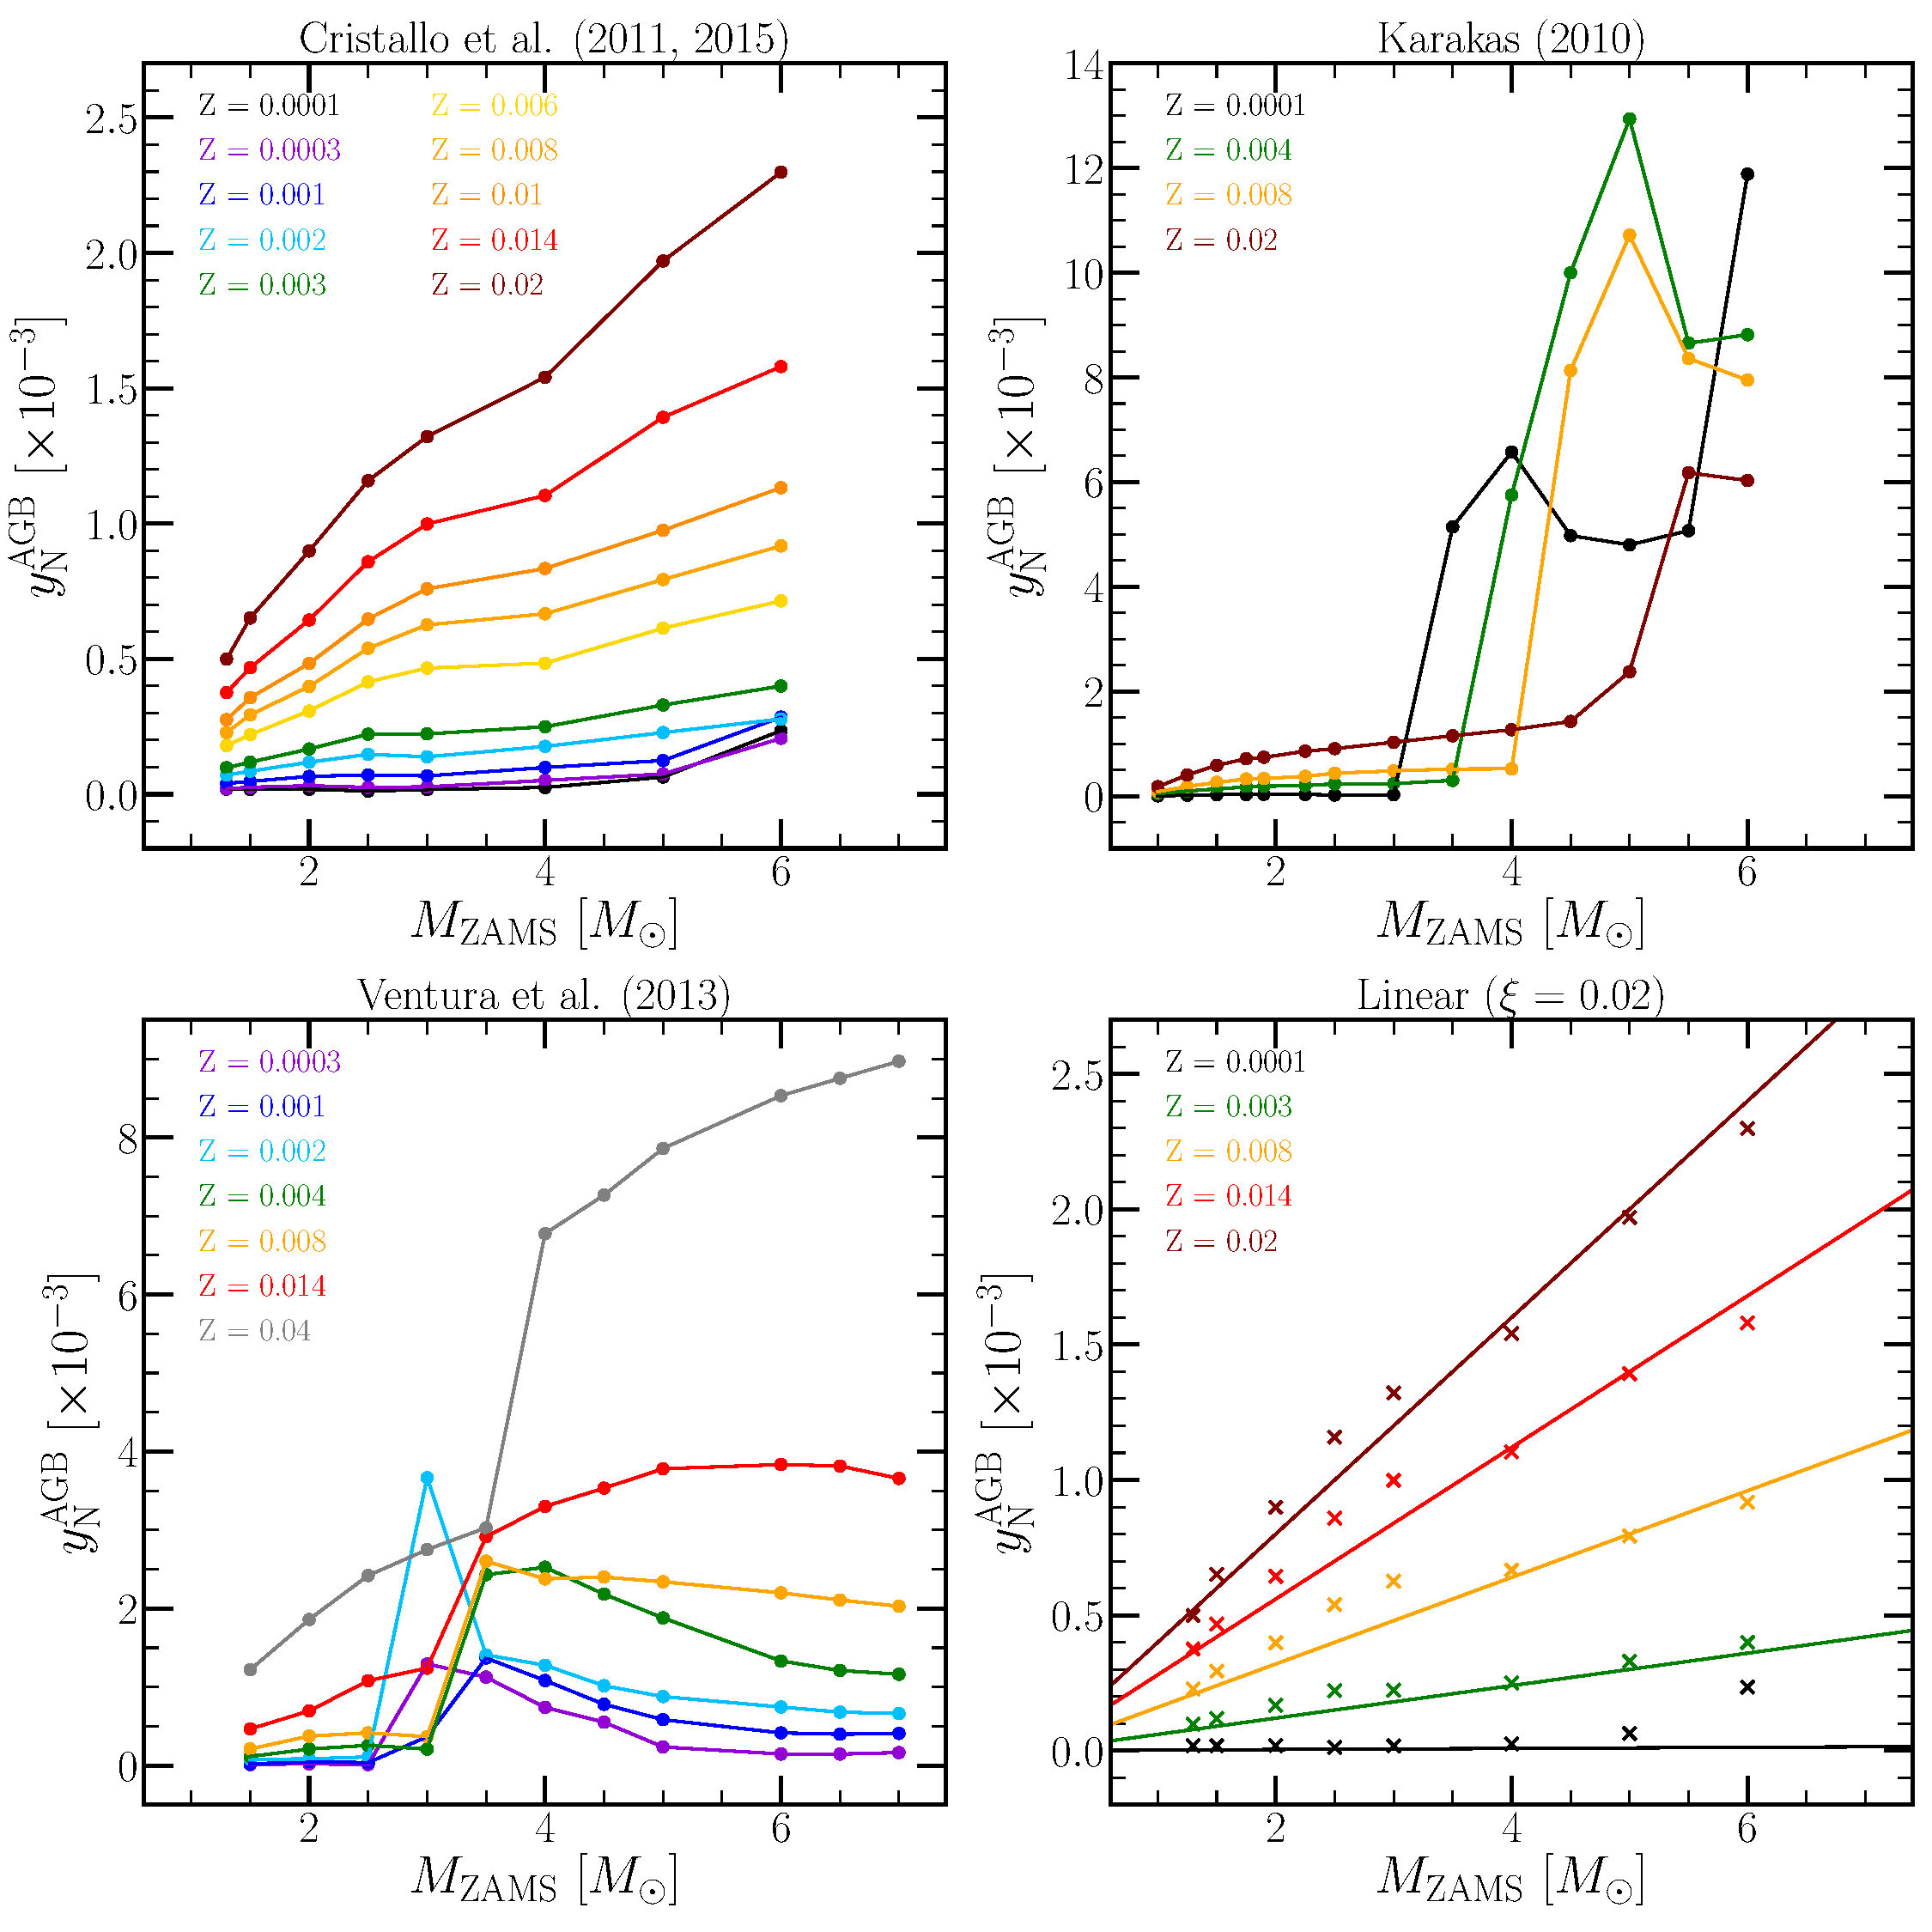
\includegraphics[scale = 0.4]{agb_yield_models.pdf} 
\caption{
The fractional yields of N from AGB stars~$y_\text{N}^\text{AGB}$ as a function 
of progenitor ZAMS mass and birth metallicity~$Z$ as reported 
by~\citet{Cristallo2011, Cristallo2015} (upper left),~\citet{Karakas2010} 
(upper right), and~\citet{Ventura2013} (lower left). In the lower right panel, 
we show the yields predicted by our linear model (colored lines; see discussion 
in~\S~X) in comparison to the~\citet{Cristallo2011, Cristallo2015} predictions 
(colored X's). 
}
\label{fig:agb_yield_models} 
\end{figure*} 

\begin{itemize} 
	\item A significant portion of N's observed abundances can be attributed 
	to yields from AGB stars~\citep{Johnson2019}. 
\end{itemize} 

\begin{figure*} 
\centering 
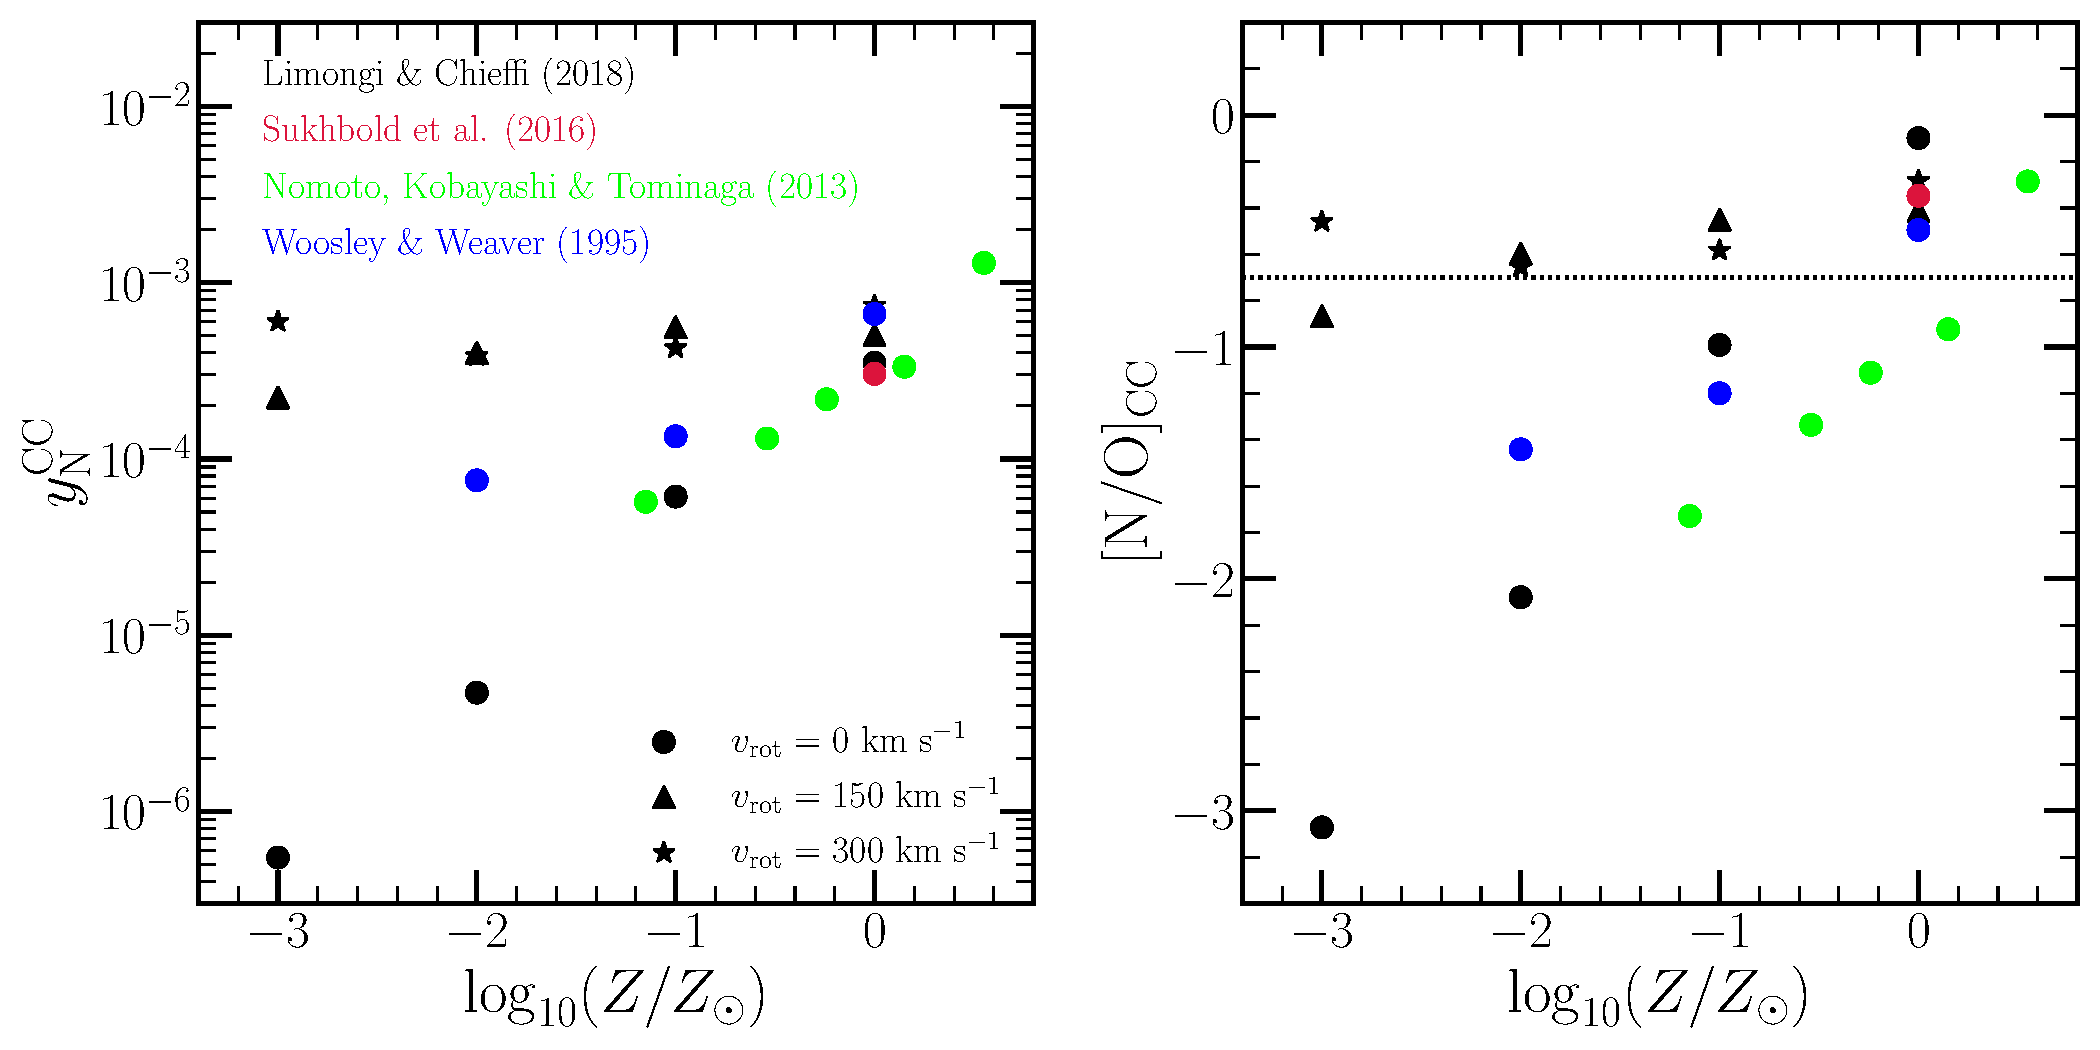
\includegraphics[scale = 0.5]{n_cc_yields.pdf} 
\caption{
\textbf{Left}: IMF-averaged CCSN yields of N calculated 
using~\vice's~\texttt{vice.yields.ccsne.fractional} function with the tables 
published by~\citet[][blue]{Woosley1995},~\citet*[][green]{Nomoto2013}, 
\citet[][red]{Sukhbold2016}, and~\citet[][black]{Limongi2018}. 
All studies report yields for non-rotating progenitors only with the exception 
of~\citet{Limongi2018}, who also report yields for progenitor rotational 
velocities of 150 (triangles) and 300 km/s (stars). 
\textbf{Right}: The [N/O] ratio predicted by each of the explosion models in 
the left-hand panel, under the same colour-coding and marker scheme. 
We mark the position of [N/O] = $-0.7$ with a black dotted line, the value 
roughly suggested by the observations of low-metallicity systems highlighted in 
Fig.~\ref{fig:no_oh_observed}. 
}
\label{fig:n_cc_yields} 
\end{figure*} 

\end{document} 
